\documentclass[sigconf,nonacm]{acmart}
\settopmatter{printacmref=false}
\renewcommand\footnotetextcopyrightpermission[1]{}
\pagestyle{plain}

\usepackage[T2A,T1]{fontenc}
\usepackage[russian,english]{babel}
\usepackage{booktabs}
\usepackage{CJKutf8}
\newcommand{\zh}[1]{\begin{CJK}{UTF8}{bsmi}#1\end{CJK}}

\begin{document}

\title{Will the Next Word Switch Language? Anticipatory Code-Switch Prediction Across 15 Language Pairs}
\subtitle{CS 6140 Machine Learning, Project Update 1 (Week 6, Fall 2026)}

\author{Artykzhan Ospan}
\affiliation{\institution{Northeastern University}\city{Seattle}\state{WA}\country{USA}}
\author{Mahamane Bachir Sadou}
\affiliation{\institution{Northeastern University}\city{Seattle}\state{WA}\country{USA}}
\author{Mukaila Rafiu}
\affiliation{\institution{Northeastern University}\city{Seattle}\state{WA}\country{USA}}

\begin{abstract}
We predict code-switching before it happens: at every token of an utterance, using only the prefix, a model
predicts whether the next token changes language and how long the new segment will last. This update
covers data engineering, labeling, a leak-free streaming loader and the first baselines on all 15 language
pairs of the SwitchLingua corpus (974,994 sentences). A logistic regression on prefix-only features reaches a
macro switch F1 of 0.555 (PR-AUC 0.528) and a duration macro-F1 of 0.531, with large gaps between pairs.
Code: \url{https://github.com/a-ospan/streaming-code-switching}.
\end{abstract}

\maketitle

\section{Problem Description}
Code-switching (CS), alternating between languages inside one utterance, is common among bilinguals, yet most
NLP work identifies languages after the whole sentence is seen. Streaming speech recognition, predictive
keyboards and dialogue agents instead need to \emph{anticipate} a switch. We formulate anticipatory CS
prediction: given only the prefix $w_1,\dots,w_t$, a causal model predicts (i) $y_{sw}\in\{0,1\}$, whether
$w_{t+1}$ is in a different language than $w_t$, and (ii) $y_{dur}\in\{$1--2, 3--6, 7+$\}$, the length in
tokens of the new segment, defined only when $y_{sw}=1$. We use the SwitchLingua text corpus~\cite{xie2025switchlingua}
and evaluate the switch F1, the duration macro-F1, and \emph{universality}: the standard deviation $\sigma$
of switch F1 across language pairs, where lower means more consistent.

\section{Background}
\textbf{Predicting switches.} Solorio and Liu~\cite{solorio2008predict} were the first to learn where a
speaker may switch, on a 40-minute Spanish--English conversation (about 8k words, 239 switches). They
trained Naive Bayes and VFI classifiers on lexical, language and POS features of only the one or two
preceding words, to suit real-time use. The best F1 was 0.28 with 96\% negative instances, which shows how
hard and imbalanced the task is. Chan et al.~\cite{chan2026predictability} ask whether word predictability
drives switch points in 1,010 Cantonese--English switches from 41 bilinguals. They regressed switching on
surprisal from autoregressive and masked language models. Less predictable words were switched more,
consistently across bilingual groups. Xie et al.~\cite{xie2025beyond} predict upcoming switches token by token
in Chinese--English dialogue (ASCEND). They compared windowed RNNs over BERT embeddings with fine-tuned mBERT
and XLM-R. mBERT reached an AUC of 0.98, but on one language pair only.

\textbf{Language identification in CS text.} Burchell et al.~\cite{burchell2024harder} test whether scalable
language identification can find CS text for corpus building. They recast it as sentence-level multi-label
tagging and compared three systems on six CS test sets. Exact-match accuracy stayed below 0.16, so no current
approach is adequate. Sterner~\cite{sterner2024english} builds one word-level tagger that separates English
from any other language. He merged five CS corpora and fine-tuned XLM-R with a named-entity head. It beat
pair-specific systems by 2.3 to 4.6 points zero-shot on unseen pairs. Kargaran et al.~\cite{kargaran2024masklid}
ask why sentence-level identifiers return only the dominant language of a CS sentence. Their training-free
MaskLID masks words of the dominant language and re-runs the identifier. Detected CS rose up to 22-fold, yet
one-word insertions were still mostly missed. Iakovenko and Hain~\cite{iakovenko2024matrix} identify the
matrix language that frames a CS utterance. They implemented Matrix Language Frame principles on text and
trained audio classifiers on those labels for Mandarin--English and Spanish--English. Their best audio systems
beat acoustic LID, but agreement between principles was sometimes low.

\textbf{Benchmarks and models for CS.} Aguilar et al.~\cite{aguilar2020lince} built LinCE, a benchmark of 11
corpora over 4 language pairs and 4 tasks (LID, NER, POS, sentiment). They report LSTM, ELMo and mBERT
baselines with a public leaderboard. It standardizes evaluation, but covers only four pairs. Khanuja et
al.~\cite{khanuja2020gluecos} built GLUECoS for Hindi--English and Spanish--English, with six tasks including
QA and NLI. They compared cross-lingual embeddings with multilingual models, also fine-tuned on synthetic CS
text. Multilingual models won, best when fine-tuned on CS data. Winata et al.~\cite{winata2021multilingual}
ask whether multilingual models handle CS. They compared them with bilingual embeddings and meta-embeddings on
NER and POS for three pairs. Pretrained multilingual models did not guarantee good CS representations.

\textbf{Multilingual backbones.} Conneau et al.~\cite{conneau2020xlmr} train XLM-R, a masked language model,
on more than two terabytes of text in 100 languages. It beat mBERT by 14.6 points on XNLI, most for low-resource languages,
but it is bidirectional, so streaming use needs a causal mask. Xue et al.~\cite{xue2021mt5} pretrain mT5 on 101
languages and balance languages with exponent-smoothed sampling. It set the state of the art on many
multilingual benchmarks; we reuse its sampling idea for unbalanced pairs. Lin et al.~\cite{lin2022xglm} train
XGLM, left-to-right multilingual language models, and evaluate few-shot learning. Their largest model beat
GPT-3 on multilingual reasoning and translation, making XGLM a natural causal backbone for us.

\textbf{Our gap.} Prior switch prediction covers one pair at a time, and CS benchmarks label switches after
the fact. We predict switches and their duration from the prefix alone, on 15 pairs at once, and measure how
consistent the predictor is across them.

\section{Dataset}
\subsection{Corpus}
SwitchLingua~\cite{xie2025switchlingua} contains 234,172 LLM-generated conversations with 19 columns (topic,
speaker profile, CS type, quality scores). The released text has \textbf{15 pairs}, more than the 12 languages
in the paper: 7 non-Latin-script pairs with English (Arabic, Cantonese, Chinese, Hindi, Japanese, Korean,
Russian), 7 Latin-script pairs with English (French, German, Italian, Malay, Filipino, Spanish, Vietnamese), and
German--French. We pin version \texttt{6e048d27} of the corpus. Generation controls are balanced by design:
50\% single-turn and 50\% multi-turn conversations; three CS types (tag, inter-sentential, intra-sentential),
each about a third; and six CS functions in equal shares. An LLM judge scored each row for fluency,
naturalness, ratio and socio-cultural fit (mean 8.42 on a 10-point scale, range 5.0 to 9.75). A
conversation holds 4.2 sentences on average, and a sentence 19.5 tokens (19.0M tokens in total). The pairs
are very unbalanced: Cantonese--English is 64\% of all sentences, while every other pair has 20k to 30k.

\subsection{Pre-processing}
\textbf{Parsing.} The text column is a stringified Python object: mostly lists of sentences, but also
dictionaries (with topic, instances, speaker or message keys), nested lists and plain strings. Our parser handles all formats and keeps text fields only, giving 974,994 sentences; 5 empty or
pasted-conversation sentences are removed and counted.

\textbf{Tokenization.} Words are split on whitespace and punctuation. Each Chinese character is one token, the
mBERT convention. A whole run of characters as one token would leak the future: a run only ends when a
non-Chinese character arrives, and 85\% of the Cantonese runs that end glued to a letter end at a switch.
Punctuation is not a token; it is kept as context for the preceding token.

\textbf{Language ID resources.} The corpus gives only each row's two languages, so we derive a language for
every token (Section~\ref{sec:labeling}). For Latin-script pairs we use the \texttt{wordfreq}
library~\cite{speer2022wordfreq}, an offline snapshot (up to about 2021) of Wikipedia, subtitle, news, book,
web and social-media text that gives each word a Zipf frequency per language. 56\% of Hindi--English rows are
romanized, so we built a romanized-Hindi lexicon (1,056 words) from the corpus itself, using the Latin words
in Devanagari rows as the English reference. Hindi is therefore reported as two strata, giving 16 evaluation
strata. As a sanity check, our per-row share of second-language tokens correlates with the ratio estimated
by the corpus's own LLM judge (Pearson 0.47 to 0.60 for 13 pairs, 0.32 for Hindi and 0.29 for Filipino, on
300 rows per pair). Since that estimate is itself noisy, a hand-validation sample of 450 sentences (30 per
pair) is prepared.

\subsection{Labeling procedure}
\label{sec:labeling}
Every sentence goes through five steps; Table~\ref{tab:example} shows the output of our code on two sentences.
\begin{enumerate}
\item \textbf{Tokenize}: words, one token per Chinese character, one token per run of digits. Punctuation is
not a token; it stays with the preceding token as context typed before the next one.
\item \textbf{Script rule}: if the token's script belongs to only one of the row's two languages, it decides.
\item \textbf{Frequency rule} (Latin-script pairs): the language whose \texttt{wordfreq} Zipf frequency is at
least 0.3 higher wins; a word below 1.0 in both lists is unknown. Romanized Hindi rows use our lexicon.
\item \textbf{Context rule}: tokens still undecided (numbers, unknown names, words frequent in both languages)
take the language of the nearest decided token, preferring the left one.
\item \textbf{Targets}: $y_{sw}(t)=1$ if the language of token $t+1$ differs from token $t$; then $y_{dur}(t)$
is the bin (1--2, 3--6, 7+) of the run of same-language tokens starting at $t+1$. The last token and
non-switch durations get no target ($-1$, ignored by the loss and the metrics).
\end{enumerate}
Labels may use the whole sentence (the context rule can look right); baseline features and model inputs never
do. Names get no special label: a name in the other script (\emph{Marvel} in Russian text) or frequent in the
other language's list counts as a switch, which the hand validation will quantify. Unit tests check every step
on hand-worked sentences.

\begin{table}[t]
\caption{Labeling output of our code on two sentences: the rule that decided each token, its language and the
targets. The comma after \emph{2022} is part of the prefix at that token.}
\label{tab:example}
\small
\setlength{\tabcolsep}{4pt}
\begin{tabular}{llccc}
\toprule
Token & Rule & Language & $y_{sw}$ & $y_{dur}$ \\
\midrule
\multicolumn{5}{l}{\emph{Spanish--English: ``Vi a Messi en 2022, honestly the best game ever!''}} \\
Vi & frequency & es & 0 & -- \\
a & context (both lists) & es & 0 & -- \\
Messi & context (unknown name) & es & 0 & -- \\
en & frequency & es & 0 & -- \\
2022, & context (number) & es & \textbf{1} & \textbf{3--6} \\
honestly & frequency & en & 0 & -- \\
the & frequency & en & 0 & -- \\
best & frequency & en & 0 & -- \\
game & frequency & en & 0 & -- \\
ever & frequency & en & -- & -- \\
\midrule
\multicolumn{5}{l}{\emph{Russian--English: \foreignlanguage{russian}{``В прошлом году} Marvel
\foreignlanguage{russian}{сняли фильм,} you know?''}} \\
\foreignlanguage{russian}{В} & script & ru & 0 & -- \\
\foreignlanguage{russian}{прошлом} & script & ru & 0 & -- \\
\foreignlanguage{russian}{году} & script & ru & \textbf{1} & \textbf{1--2} \\
Marvel & script (name) & en & \textbf{1} & \textbf{1--2} \\
\foreignlanguage{russian}{сняли} & script & ru & 0 & -- \\
\foreignlanguage{russian}{фильм,} & script & ru & \textbf{1} & \textbf{1--2} \\
you & script & en & 0 & -- \\
know & script & en & -- & -- \\
\bottomrule
\end{tabular}
\end{table}

\subsection{Splits}
\begin{table}[t]
\caption{Fixed splits, by conversation and stratified by stratum.}
\label{tab:splits}
\small
\begin{tabular}{lrrr}
\toprule
Split & Conversations & Sentences & Target positions \\
\midrule
Train (80\%) & 187,329 & 778,867 & 14.4M \\
Validation (10\%) & 23,418 & 98,046 & 1.8M \\
Test (10\%) & 23,422 & 98,081 & 1.8M \\
\bottomrule
\end{tabular}
\end{table} We split 80/10/10 \emph{by conversation}, stratified by stratum with a
fixed seed, and keep conversations sharing a sentence (5,586 duplicates) in one split (Table~\ref{tab:splits}). Table~\ref{tab:data} and Figure~\ref{fig:dur} summarize the labels. Switches are rare (5 to
13\% of positions for most pairs), so we report F1 and PR-AUC rather than accuracy.

\begin{table}[t]
\caption{Sentences and switch rate per stratum (all splits).}
\label{tab:data}
\small
\begin{tabular}{lrr}
\toprule
Stratum & Sentences & Switch rate \\
\midrule
Chinese--English & 29,561 & 5.1\% \\
Japanese--English & 27,893 & 6.3\% \\
Cantonese--English & 619,863 & 6.8\% \\
Italian--English & 24,165 & 8.4\% \\
German--French & 23,598 & 8.6\% \\
Arabic--English & 26,791 & 9.1\% \\
Vietnamese--English & 26,803 & 9.1\% \\
Russian--English & 24,625 & 9.3\% \\
Spanish--English & 24,517 & 9.6\% \\
German--English & 19,583 & 9.8\% \\
French--English & 23,563 & 10.3\% \\
Korean--English & 25,388 & 10.6\% \\
Malay--English & 26,127 & 13.3\% \\
Hindi--English (Devanagari) & 11,186 & 16.1\% \\
Filipino--English & 25,826 & 19.1\% \\
Hindi--English (romanized) & 15,505 & 31.4\% \\
\bottomrule
\end{tabular}
\end{table}

\begin{figure}[t]
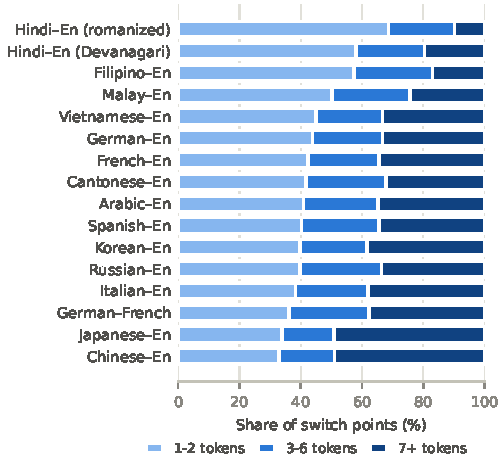
\includegraphics[width=\columnwidth]{figures/duration_mix.pdf}
\Description{Stacked horizontal bars per stratum showing the share of switch points whose new segment lasts 1-2, 3-6 or 7+ tokens.}
\caption{Duration class of the segment after a switch, per stratum. Hindi and Filipino are dominated by short
insertions; Chinese and Japanese segments, counted in characters, are often 7+.}
\label{fig:dur}
\end{figure}

\section{Experimentation and Results}
\subsection{Streaming setup}
At token $t$ the input is the prefix only. For transformers, each sentence is encoded once with the model's
subword tokenizer and the prediction for word $t$ is read at the last subword that ends before word $t+1$. A
position is skipped if a subword spans the boundary or if the prefix tokenizes differently on its own, so no
future character can leak; automated tests change every word after $t$ and check that inputs at $t$ do not
change. To keep Cantonese from dominating training, pairs are drawn with probability proportional to
$n_p^{0.3}$, as in mT5~\cite{xue2021mt5}, which lowers Cantonese from 64\% to 16\% of samples.

\subsection{Baselines}
\textbf{Majority class} always predicts no switch and the most frequent duration (1--2). \textbf{Logistic
regression} uses prefix-only features: current language, length of the current run, switches so far,
position, punctuation typed after the token, script, stratum, and stratum $\times$ current language. Tags are
rebuilt from the prefix only, since the context rule may look right. A binary model predicts $y_{sw}$ and a
multinomial (softmax) model predicts $y_{dur}$, trained on true switch points. Both use 3,000 training
sentences per stratum (838k positions); the switch threshold (0.225) is tuned on training data. All results
are on the validation split (1.8M positions), macro-averaged over the 16 strata.

\begin{table}[t]
\caption{Baselines on the validation split (macro average over 16 strata). $\sigma$: standard deviation of
switch F1 across strata.}
\label{tab:base}
\small
\setlength{\tabcolsep}{4pt}
\begin{tabular}{lrrrrrr}
\toprule
Model & F1 & PR-AUC & P & R & $\sigma$ & Dur.\ F1 \\
\midrule
Majority & 0.000 & 0.114 & 0.000 & 0.000 & n/a & 0.202 \\
Logistic reg. & \textbf{0.555} & \textbf{0.528} & 0.550 & 0.571 & 0.076 & \textbf{0.531} \\
\bottomrule
\end{tabular}
\end{table}

\begin{figure}[t]
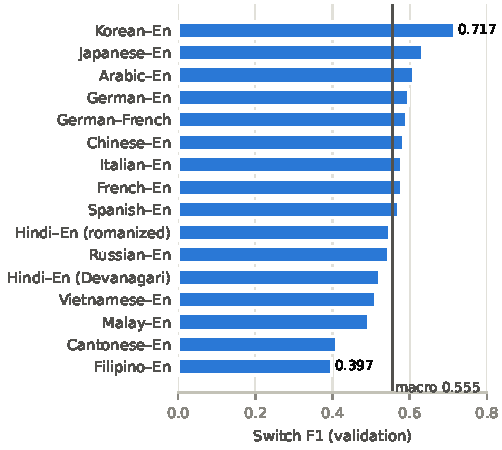
\includegraphics[width=\columnwidth]{figures/baseline_f1.pdf}
\Description{Horizontal bars of logistic regression switch F1 for 16 strata, from Filipino-English (0.397) to Korean-English (0.717), with a vertical line at the macro average 0.555.}
\caption{Logistic regression switch F1 per stratum (validation). The line is the macro average.}
\label{fig:f1}
\end{figure}

\subsection{Results}
Table~\ref{tab:base} shows the logistic regression far above the majority class, with balanced precision and
recall. Figure~\ref{fig:f1} shows large gaps between pairs: Korean (0.717) and Japanese (0.633) are easiest,
Filipino (0.397) and Cantonese (0.409) hardest, giving $\sigma=0.076$.

\textbf{Why Korean is easy and Cantonese hard.} The strongest feature is punctuation (Table~\ref{tab:punct}).
In Korean, Chinese and Japanese, 68 to 70\% of switches follow a comma or sentence end, versus 2 to 4\% of
other positions. In Cantonese only 38\% do: English words are inserted mid-clause (\zh{呢個}IG
update\zh{好正}), with no visible cue. The baseline thus learns clause-level switching but not insertions.

\begin{table}[t]
\caption{Share of positions right after punctuation (2,500 validation sentences per pair) and baseline switch F1.}
\label{tab:punct}
\small
\setlength{\tabcolsep}{4pt}
\begin{tabular}{lrrr}
\toprule
Pair & Switches & Other positions & Switch F1 \\
\midrule
Korean--English & 68.6\% & 2.4\% & 0.717 \\
Japanese--English & 69.9\% & 3.7\% & 0.633 \\
Chinese--English & 67.5\% & 3.4\% & 0.584 \\
Cantonese--English & 38.0\% & 5.5\% & 0.409 \\
\bottomrule
\end{tabular}
\end{table}

\textbf{Duration.} Short (1--2) and long (7+) segments are recognized well (87\% and 69\% recall), but only
13\% of 3--6 segments are (Table~\ref{tab:cm}), since prefix features cannot tell a phrase from a clause.

\begin{table}[t]
\caption{Duration confusion matrix of the logistic regression at true switch points (validation, all strata).}
\label{tab:cm}
\small
\begin{tabular}{lrrrr}
\toprule
True $\backslash$ predicted & 1--2 & 3--6 & 7+ & Recall \\
\midrule
1--2 & \textbf{56,337} & 3,011 & 5,777 & 86.5\% \\
3--6 & 17,264 & \textbf{4,737} & 14,357 & 13.0\% \\
7+ & 10,395 & 3,914 & \textbf{31,844} & 69.0\% \\
\bottomrule
\end{tabular}
\end{table}

\textbf{Tokenizer alignment.} We checked how the streaming loader fits each backbone's tokenizer on 300
training sentences per stratum (Table~\ref{tab:align}). In Chinese-character text, 20 to 30\% of character
positions fall inside one XLM-R subword and are skipped, but no true switch point is lost. XGLM lacks common
Cantonese characters (5.4\% unknown subwords) and loses 4 to 5\% of switch points in Chinese and Cantonese.
All other strata keep at least 96\% of positions with both tokenizers. Later model comparisons will therefore
use positions valid for both models.

\begin{table}[t]
\caption{Usable prediction positions per tokenizer (lowest strata) and XGLM unknown-subword rate.}
\label{tab:align}
\small
\setlength{\tabcolsep}{4pt}
\begin{tabular}{lrrr}
\toprule
Stratum & XLM-R & XGLM & XGLM unknown \\
\midrule
Chinese--English & 68.9\% & 75.2\% & 0.6\% \\
Japanese--English & 78.4\% & 85.3\% & 0.2\% \\
Cantonese--English & 79.6\% & 85.3\% & 5.4\% \\
Korean--English & 99.9\% & 95.8\% & 0.6\% \\
\bottomrule
\end{tabular}
\end{table}

\section{Plan for Next}
Week 7: causal masking and the two prediction heads, already implemented with a test showing that later
tokens cannot change earlier outputs. Weeks 8 to 10: multitask training of XLM-R with a causal
mask~\cite{conneau2020xlmr} and the natively causal XGLM~\cite{lin2022xglm}, tuning the loss weights,
comparing sampling exponents 0.3 and 0, and comparing backbones against these baselines. Weeks 11 and 12:
per-pair evaluation, universality $\sigma$ and bootstrap confidence intervals, and hand validation of the
language tags. Weeks 13 and 14: error analysis by script and switch type, the streaming demo and the final
paper.

\bibliographystyle{ACM-Reference-Format}
\bibliography{references}

\end{document}
